% !TEX TS-program = XeLaTeX
% use the following command:
% all document files must be coded in UTF-8
\documentclass[english]{textolivre}
% build HTML with: make4ht -e build.lua -c textolivre.cfg -x -u article "fn-in,svg,pic-align"

\journalname{Texto Livre}
\thevolume{15}
%\thenumber{1} % old template
\theyear{2022}
\receiveddate{\DTMdisplaydate{2022}{7}{17}{-1}} % YYYY MM DD
\accepteddate{\DTMdisplaydate{2022}{7}{31}{-1}}
\publisheddate{\DTMdisplaydate{2022}{9}{21}{-1}}
\corrauthor{Paula Aguadero Ruiz}
\articledoi{10.35699/1983-3652.2022.40506}
%\articleid{NNNN} % if the article ID is not the last 5 numbers of its DOI, provide it using \articleid{} commmand 
% list of available sesscions in the journal: articles, dossier, reports, essays, reviews, interviews, editorial
\articlesessionname{dossier}
\runningauthor{Aguadero Ruiz} 
%\editorname{Leonardo Araújo} % old template
\sectioneditorname{Daniervelin Pereira}
\layouteditorname{Leonado Araújo}

\title{Cognitive neuroscience: improvement of autonomous thinking in reading through video games}
\othertitle{Neurociência cognitiva: melhoria do pensamento autônomo na leitura através de videogames}
% if there is a third language title, add here:
%\othertitle{Artikelvorlage zur Einreichung beim Texto Livre Journal}

\author[1]{Paula Aguadero Ruiz \orcid{0000-0001-5899-6267} \thanks{Email: \href{mailto:par00013@red.ujaen.es}{par00013@red.ujaen.es}}}
\affil[1]{Universidad de Jaén, Facultad de Humanidades y Ciencias de la Educación, Departamento Pedagogía, Jaén, España.}

\addbibresource{article.bib}
% use biber instead of bibtex
% $ biber article

% used to create dummy text for the template file
\definecolor{dark-gray}{gray}{0.35} % color used to display dummy texts
\usepackage{lipsum}
\SetLipsumParListSurrounders{\colorlet{oldcolor}{.}\color{dark-gray}}{\color{oldcolor}}

% used here only to provide the XeLaTeX and BibTeX logos
\usepackage{hologo}

% if you use multirows in a table, include the multirow package
\usepackage{multirow}

% provides sidewaysfigure environment
\usepackage{rotating}

% CUSTOM EPIGRAPH - BEGIN 
%%% https://tex.stackexchange.com/questions/193178/specific-epigraph-style
\usepackage{epigraph}
\renewcommand\textflush{flushright}
\makeatletter
\newlength\epitextskip
\pretocmd{\@epitext}{\em}{}{}
\apptocmd{\@epitext}{\em}{}{}
\patchcmd{\epigraph}{\@epitext{#1}\\}{\@epitext{#1}\\[\epitextskip]}{}{}
\makeatother
\setlength\epigraphrule{0pt}
\setlength\epitextskip{0.5ex}
\setlength\epigraphwidth{.7\textwidth}
% CUSTOM EPIGRAPH - END

% LANGUAGE - BEGIN
% ARABIC
% for languages that use special fonts, you must provide the typeface that will be used
% \setotherlanguage{arabic}
% \newfontfamily\arabicfont[Script=Arabic]{Amiri}
% \newfontfamily\arabicfontsf[Script=Arabic]{Amiri}
% \newfontfamily\arabicfonttt[Script=Arabic]{Amiri}
%
% in the article, to add arabic text use: \textlang{arabic}{ ... }
%
% RUSSIAN
% for russian text we also need to define fonts with support for Cyrillic script
% \usepackage{fontspec}
% \setotherlanguage{russian}
% \newfontfamily\cyrillicfont{Times New Roman}
% \newfontfamily\cyrillicfontsf{Times New Roman}[Script=Cyrillic]
% \newfontfamily\cyrillicfonttt{Times New Roman}[Script=Cyrillic]
%
% in the text use \begin{russian} ... \end{russian}
% LANGUAGE - END

% EMOJIS - BEGIN
% to use emoticons in your manuscript
% https://stackoverflow.com/questions/190145/how-to-insert-emoticons-in-latex/57076064
% using font Symbola, which has full support
% the font may be downloaded at:
% https://dn-works.com/ufas/
% add to preamble:
% \newfontfamily\Symbola{Symbola}
% in the text use:
% {\Symbola }
% EMOJIS - END

% LABEL REFERENCE TO DESCRIPTIVE LIST - BEGIN
% reference itens in a descriptive list using their labels instead of numbers
% insert the code below in the preambule:
%\makeatletter
%\let\orgdescriptionlabel\descriptionlabel
%\renewcommand*{\descriptionlabel}[1]{%
%  \let\orglabel\label
%  \let\label\@gobble
%  \phantomsection
%  \edef\@currentlabel{#1\unskip}%
%  \let\label\orglabel
%  \orgdescriptionlabel{#1}%
%}
%\makeatother
%
% in your document, use as illustraded here:
%\begin{description}
%  \item[first\label{itm1}] this is only an example;
%  % ...  add more items
%\end{description}
% LABEL REFERENCE TO DESCRIPTIVE LIST - END


% add line numbers for submission
%\usepackage{lineno}
%\linenumbers

\begin{document}
\maketitle

\begin{polyabstract}
\begin{abstract}
With the objective to demonstrate the real hidden capacities of reading in students with difficulties of learning such as dyslexia with the use of videogames, we have carried out a study with grammar education students. In order to do this, we have revised some literature to present and justify the real case study of an 8-year-old child with reading difficulties. Videogames have been used to show how he has improved his learning. To do this, we have tested his capacities with a standarized reading test (DIP-le) and we have done a follow-up with a videogame called DytectiveU, which is supposed to overcome his dyslexia. We have verified, with he same test, that the more the child plays this game, the better reading capabilities and abilities he develops. Finally, we demonstrate and verify the benefits of using videogames in psycopedagogical diagnosis and psycopedagogical tracing. We expect to increase the use of videogames in psycopedagogical clinics due to their great benefits.

\keywords{Innovation \sep Reading \sep Reading difficulties \sep Videogames \sep Autonomous thinking}
\end{abstract}

\begin{portuguese}
\begin{abstract}
Com o objetivo de demonstrar as altas capacidades de leitura em alunos com dificuldades de aprendizagem, como a dislexia com o uso de videogames, realizamos uma pesquisa com alunos do Ensino Fundamental. Para isso, revisamos parte da literatura a fim de apresentar e justificar um estudo de caso real de uma criança de oito anos com dificuldades de leitura. Os videogames têm sido usados para constatar como ele melhorou seu aprendizado. Para isso, testamos suas capacidades com um teste padronizado (DIP-le) de leitura e fizemos um acompanhamento com um videogame chamado DytectiveU, que deve superar sua dislexia. Constatamos com o mesmo teste que quanto mais a criança joga esse jogo, melhores capacidades e habilidades de leitura ela desenvolve. Por fim, demonstramos e constatamos os benefícios do uso de videogames no diagnóstico psicopedagógico e no rastreamento psicopedagógico. Esperamos aumentar o uso de videogames nas clínicas psicopedagógicas devido aos seus grandes benefícios.

\keywords{Inovação \sep Leitura \sep Dificuldades de leitura \sep Videogames \sep Pensamento autônomo}
\end{abstract}
\end{portuguese}
% if there is another abstract, insert it here using the same scheme
\end{polyabstract}

\section{Introduction: reading as an act of interpretation}\label{sec-intro}
\subsection{Some elements to understand the logical aspects of reading}
The approach to reading as a skill set began to be questioned in the late sixties with the advancement of psycholinguistics and cognitive psychology. From that moment on, the possible ways of understanding the reading processes are reformulated. According to the basic postulate of equilibrium theory, it is possible to characterize knowledge as a process of interaction between the subject and the object. In the case of reading, the subject is confronted with an object different from himself constituted by written language, and with it he must interact assimilating it to his previous schemes and adjusting the latter to the peculiarities of it. We consider that this interaction is adaptive when there is construction of meanings (Here adaptation is taken in the Piagetian sense, considering adaptation as a process of balancing synthesis). Reading is not simply spelling or deciphering, but it consists of a series of transactions in which the subject tries to construct a possible meaning of the text \cite{goodman_proceso_1980}. The reading process employs a series of strategies, that is, schemes that are put into play to obtain, evaluate and use the information. We will write them following Goodman.

There are, for example, sampling strategies. The text provides indexes that are not all equally useful. The reader should select from these indexes only those that are most useful for obtaining meaning from the text. If the reader used all the available indexes, without the possibility of selecting and hierarchizing the afferences, he would be overloaded with unnecessary or irrelevant information. Prediction strategies are also used to anticipate the end of a word or story, the structure of a sentence, etc. The speed of the reading shows that the reader is sampling and predicting while reading, since he would not be able to work with so much information if he had to process all the indexes. The subject predicts on the basis of the indexes from the sampling of the text, and does that sampling on the basis of his predictions. Sometimes we make predictions that later turn out to be false, or we make unsubstantiated inferences. Constant self-control is necessary through the use of confirmation strategies, which allow ratifying or rejecting the predictions and inferences made. Reading is tantamount to a constant rethinking and revisiting the text with an alternative hypothesis. When the subject cannot confirm their expectations, they use their self-correction strategies to reconsider the information they have or obtain more information.

From this point of view, we can say that reading is not only a visual process, since it is the inferential procedures that allow us to anticipate, for example, what kind of word will come next, and can even be used to decide what the text should say when there is a printing error. That is to say, in reading there is an interaction between two types of information: visual information (provided by the visual exploration of the perceptual indexes provided by the text) and non-visual information (provided by the reader's previous linguistic and thematic knowledge that allows him to assimilate and interpret the information obtained through perceptual mediation). Aspects of subjective positioning in front of the text as an object could be included in the category of non-visual information, influencing the construction of the meaning of the written.

In short, when reading the subject confronts his previous certainties (non-visual information) with the characters of the object (visual information). He develops a hypothesis of the meaning of the text,  doubts what was thought, verifies it; with these demands the subject who reads is confronted, a confrontation in which his strategies constitute specific modes of a singular approach. Through this brief exposition of the procedural aspects of reading, we will understand how the cognitive modality is updated in the subjective and singular approach that each subject makes towards this external object that is the written text.

\subsection{Reading and cognitive modality}\label{sec-normas}
The concept of cognitive modality refers to the result of the testing of the consistency that the relationship between the statements offered to the child by the other significant ones with their concomitant libidinal investments is acquired, and what it supposes as the intelligible causes of an object \cite{wettengel_produccion_1995}. The problem of reading refers to the relationship of the subject with the discourse of the other, whose statements account for their desire.

In the origins, the discourse that directs towards the child who exercises the maternal function, anticipates the senses that the infants cannot build by their natural prematureness. Through primary violence \cite{aulagnier_violencia_1975}, the mother imposes on the child's psyche thoughts, actions and meanings that are supported by the registration of the need of the infant but imposed from the record of the unconscious desire of the Other. In this way a logic of desire is established: the relationship with the world is organized according to the omnipotence of the maternal desire. Desire constitutes the foundation of the truth of the statements, since the subject attributes a character of certainty to the contents of the discourse enunciated by the Other. This guarantee of certainties offered by the Other expires in the subject gradually and concomitantly with the installation of doubt, otherness, absence. We are already in the register of the secondary. Here the test of truth will not be sustained by the omnipotent desire of the Other but by the discourse as a whole. Curiosity, doubt, the desire to know, suppose the abandonment of the original certainties and the ability to tolerate uncertainty to launch a process of search and construction of new possible senses, that is, of a gain of future pleasure in the form of provisional truth substitute for the lost certainties.

The subject's relationship with the text seems to refer to the modalities of his relationship with the discourse of the Other. Some children cannot doubt the text, they consider it as a source of unquestionable truth, they place meaning as a pre-existing object within the text, and they position themselves in front of it as recipients of a truth whose certainty is guaranteed by the one who enunciates it. We cannot say that such an operation is that of reading, since reading involves the construction of senses and not their decipherment. To be able to read, the subject needs to place himself in front of the text in a different positioning than the search for a truth, he needs to take into account the text in its otherness, in its difference, tolerate the uncertainty and ignorance that the text puts in evidence, catechize its own constructive possibilities, look for in the text elements of information that allow to initiate a process of construction of meanings, constantly doubt what he finds in that material, elaborate hypotheses of possible meanings, verify them. We will call the set of such operations reading.

\subsection{Where playing was, reading must come}\label{sec-conduta}
According to Winnicot, the location of the cultural experience – like play – is the potential space that exists between the individual and the environment. The cultural experience begins with the creativity of the game. The game takes place in a transitional space, existing between the subjective object and the object perceived objectively, that is, between the self and the non-self.

Everything that remains linked to the desiderative force of the game is located within this intermediate zone of experience. On the contrary, those activities that remain unconsciously detached from the playful register appear deprived of impulsive roots. They conform to the service of the superego, giving rise to situations of dissatisfaction in the form of instrumental failure or relative success  but without concomitant pleasure. As you will see, we are moving away from an adaptationist perspective. From our point of view, reading, and learning in general, have little to do with adaptation. The only criterion to be able to speak of a subjective learning is if libidinal circulation can be discovered there. That is, deployment of desire, which by definition brings it closer to the playful register. A child can read perfectly from the adaptive-instrumental point of view endorsed by the school, but nevertheless, this pseudo-learning can be revealed as purely inappropriate for him. Inappropriate in the sense that there is no subjective appropriation of the processes that reading entails, nor pulsional circulation that crosses reading. There may be family desire that takes the subject, producing an impoverishment in which learning in general is captured in an overadaptive system at the service of the desire of the Other.

We prefer to use the substantive infinitive – to read – instead of the noun reading, in the same sense that Winnicot differentiates the game from playing, thus enhancing its character as a significant process and operation. Reading is meaningless if it is not a corollary and heir to playing. If reading and playing are separated, the desiring movement is excluded from the learning processes, and the entire secondary process, disjunct from the libidinal circulation that energizes it. Returning to the famous Freudian formula: Wo es war, soll Ich werden (where the It was, the I must come), it is possible to argue that one of the most decisive tasks in terms of learning is the transformation of the playful order as a significant production in what will later be reading and learning in general: Where playing was, reading must come. \textcite{casas_de_pereda_en_1999} defines significant production in relation to the habilitation of psychic inscription and the circulation of desire.

The purpose is to think about the game and symbolization. Play, as part of children's discourse, constitutes a true work of psychic organization that entails significant production in a bodily and linguistic modality at the same time. It is the very multifaceted character of children's discourse, which includes movement and voice even outside of articulated language. And this significant production alludes to the psychoanalytic signifier that, like a two-sided coin, looks at the body and the symptom, the gesture and the word, in a process in which it will become necessary to discriminate the symbol, the symbolic, the symbolization. Significant production, then, that enables and establishes, at the same time, the psychic inscription and the circulation of desire. Production that also entails the possibility that the sign becomes a symbol and that the singularity appears, that is, a moment of subjectivity (which makes the historization of the subject).

Such an event would be the result of a shared experience. I think that, in his constitutive helplessness, the child needs the other so that the sign becomes a symbol, that of the surrounding universality, of the real to be apprehended, can be passed, in that moment of apprehension-symbolization, to the mark, symbol that constitutes from then on its singularity; from the world to the personal, from the sign to the symbol. Symbolization, as work on absence, is unconscious articulation, presence of the subject of the unconscious.  \cite{casas_de_pereda_en_1999}.

In effect, it is a process that turns the sign into a symbol and allows the emergence of the singularity. Just as when playing the child transforms an in-significant object, even a disposable object, subjectivizing it and giving it the status of a toy, also when reading the subject transmutes the real into a signifier. Transform stains into letters. Reading is all about this process of subjective transformation, and from there its constructive vicissitudes arise. It is not about annihilating the game to make way for the work of reading, writing and learning in general. Just as the Self is altered by receiving the contents of the unconscious, by reflecting them and trying to put into action its impulses, reading receives from its precursors - playing - the pulsating dynamism of subjective processes. It is then that the formations of desire developed in the field of play give their strength to learning as a central activity of latency, thus conferring on it the pulsional base necessary for its deployment. Without this dynamic basis, reading is not established, it constitutes only an activity that is perhaps technically acceptable but empty of subjective significance.

Many times does the curricular order go against these processes of subjectivation that we postulate as necessary for the constitution of the possibility of reading. So Javier, a six-year-old boy, will tell us, at the beginning of his first year of schooling: The Miss told us that now we are not going to play anymore as we played in Preschool. To play there is recess, in the class you have to learn. Here Javier teaches us a lot. For the education system there is a structural disjunction between playing and learning. It would almost seem that this is one of the basic oppositions that govern the curricular order. If you play, you don't learn. If you learn, you don't play. And in school you learn. Learning then is detached from the desiring movement and elevated to a categorical imperative, with the depersonalization and inflexibility of the signifiers of the superego in the class you have to learn.

\subsection{The principle of difference}\label{sec-fmt-manuscrito}
In order to be able to read, the text must be assured of its own existence. It is necessary that the text is shown in its difference and that the subject considers it in its otherness and in its autonomous literality. But, in addition, after having been able to recognize the otherness of the text to which it is directed, the reading should develop a reflection also autonomous and differentiated. Any annulment of the differences between the subject and the text would result in a symptomatic reading. If the text is not considered in its difference, in its literality, the reading becomes a simple projective display of the reader's fantasy. If the text is not allowed to assert itself in its particular properties, the reading pretends an impossible: the illusory annexation of the subject's undifferentiated text.

If, on the other hand, one falls into a focus on the text, the risk is dogmatism that, in the words of \textcite{hornstein_aulagnier:_1994}, replaces the impulse to know with the desire to house what has already been thought of by another. This intolerance of the difference of the text is a consequence of narcissism that feels the other as threatening. To be able to read, it is necessary to tolerate the difference with which the text opposes us. This position is impossible for a subject who tries to preserve a narcissistic place (in which case we would witness a disqualification of the text) and for those who seek in the real a guarantee of certainties that preserve it under the protection of an illusory truth (in which case we would observe a production focused on the already-written).

To be able to read, it is necessary that the psyche – far from preserving narcissism and inertia – becomes a generator of difference \cite{derrida_gramatologi_1967}.  If the apparatus aspires to null excitation, the text considered as a disturbance to be eliminated will be denied, ignored, metabolized into the same-proper to defend itself from the disturbance implied by its otherness. The reader, on the other hand, is a seeker and producer of differences rather than an inertial defender.

\subsection{The forms of textual positioning}\label{sec-formato}
We will call positioning the foundation that regulates these forms of textual processing possible for the subject. That is, the operations that the child is able to perform on the text are not random, but are regulated by a system that enables certain forms of action and limits others and organized through said system. Repeating, opining, dialoguing, thinking, are revealed as the paradigmatic operations that establish the order in which the subject is located with respect to the text.  Positioning refers to what the subject attributes to himself as a right to do in relation to what is written.

\begin{enumerate}[label=\alph*.]
    \item Glosators: If the child can only repeat what the text says, and is unable to think with it beyond what is written, he is placed in a particular way in relation to the written language. It seems that for this subject the text is erected in a preponderant position. From the written emanates the truth; thought is reduced to repetition, reflexive autonomy annulled, imagination relegated. We will not say that this child is able to read, even if there is a correct sound before the text. The indemnity of the instrumental mechanisms of reading does not guarantee their subjective appropriation. Their actions remind us of the operation that in times of medieval Christianity was carried out on sacred texts. We will say then that it acts as a glossator of the text. The gloss is not reading but uncritical commentary. The text thus turned into dogma is elevated to the category of absolute truth. From this character attributed to the text derives the truth of its statements and not vice-versa.
    \item Doxists: At the other extreme, there are children who cannot read either, but not because they reserve the text a place of revealed truth, but because they cannot question their own certainties. This process assumes that literal information is dismissed in favor of prior knowledge, and the interpretation of the text is forced to conform to the above concepts. Faced with a question of understanding, the child -positioning himself as a doxist- will opine; that is, he will make a personal comment and not an inference resulting from the synthesis between the information provided by the text and the knowledge of the reader. In this solipsistic operation the text loses the autonomy of its literality, ceases to be such and becomes the child's spokesman. It does not say what the author wrote but what the subject wants him to say. Nor can we call this manipulation of the text reading. We will say instead that it is doxa, in the Platonic sense. Doxa is a form of knowledge based on opinion, without empirical support or the possibility of contrast. The guarantee of truth in the doxa is given by the subject who enunciates it, who claims certainty. The text is degraded in its literality, forgotten and descended to the rank of pre-text for the imaginary unfolding of the subject.
    \item Readers: Only the position of reader supposes in the subject the construction of the autonomy of thought necessary to dialogue with the text. Question their own certainties in a process of constant testing, take into consideration what is written in their difference, not as a single truth but as a possibility of thinking. In this way, the text becomes an interlocutor, a carrier of ideas that can provide elements with which the subject builds his own thoughts. The position of reader is a corollary of the autonomy of thought. Through the possibility of doubting what is thought, the investment of the voice that enunciates is separated from the investment of what is enunciated. In this way the reader does not limit himself to accepting the text as truth or rejecting it as false for the pleasure or suffering it causes him but the statements will be put to the test.
\end{enumerate}

\section{Method. Results}\label{sec-modelo}
To take a clinical cut that illustrates some of the topics addressed, consider the case of Mariano (not his real name), an 8-year-old boy who has learning difficulties in the area of reading. I will not present the entire diagnosis but only a functional selection to the thematic cut-out that I propose. Let's start by referring to the production read by the child during the Positional Diagnosis in Reading and Writing (DIP-le). Mariano reads: Un dí-a, el due-ño de la culesita (sic) … calesita se dio cuen... cuenta. Dice que el ca...ca-ballo Valentin se había roto una de sus petas (sic) ...patas de madera”. According to the perspective that we have been developing, we can ask ourselves about the modalities of construction of senses in this child. Anticipation strategies seem deficient as Mariano is unable to foresee the meaning of the word he will read next while he is embarked on the reading. However, he can self-correct, accounting for control strategies appropriate to the production of meaning. Below (\Cref{fig01}) I show the written informed consent (in Spanish, because they are native speakers). Note: I have erased her personal data, such as her complete name, her ID (Spanish, DNI) and her signature.

\begin{figure}[htbp]
 \centering
 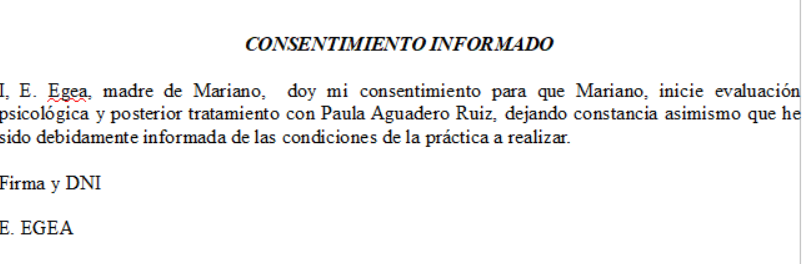
\includegraphics[width=0.85\textwidth]{Fig1.png}
 \caption{Written informed consent.}
 \label{fig01}
 \source{Own elaboration.}
\end{figure}

The possibility of inferential anticipation is an extremely complex strategy since it involves an articulation of textual levels intertwined with each other. Words, text and context are elements that only to a naïve observer will seem isolated. We understand the phrase from the meaning of the words at the same time that the meaning of the words crystallizes according to the one that emerges from the sentence. The same goes for sentences and text. In this sense, there is an articulation of hierarchical levels between these three elements that becomes a condition of possibility of reading. That is to say that the difficulty of anticipation speaks to us of a disruption of the hierarchical levels between word, phrase and text.

The phrase read by the child is a fragment of a story that he must read aloud as part of the test situation. At the end of the reading, he is asked questions of retention - which Mariano answers appropriately - and inference. In this last point a significant answer appears. The text does not clarify whether one of the characters (the carpenter) is young or old, but this data can be inferred from clues that are provided. Mariano affirms that the carpenter is old, because those who are old like horses because they used to have horses. This statement does not recover indications that the text provides, but it is an opinion of the child.

We categorize this particular mode of response as doxa. Answers of the same order are given in situations of silent reading and read by the interviewer. That is, the child cannot differentiate his own previous knowledge from that information that the text provides. It makes the text say something that wasn't there. The violence. It will be necessary to resort to the discourse of parents in search of elements that can help us to resignify this situation. Allow me to select – from the totality of the parents' discourse in the interviews carried out – only some significant fragments based on the proposed cutout, not to close a diagnosis of the child but only to return to the concepts developed. Referring to the reason why they consult, the child's mother says: Mariano apparently because of what the teacher says he does not pay attention, he ignores her. With me he also forgets things, he has a hard time concentrating when he reads. He looks at you but doesn't attend to you. He’s scattered.

Reading difficulties are frequently associated with attentional problems. From our point of view, the attentional process involves object investing. Mariano seems to have difficulties in the possibility of investing cultural objects: paying attention and reading are in fact complex sublimatory processes. In addition, the maternal discourse equates two terms: (does not pay attention, and ignores [the teacher]), which appear meanings as synonyms.

For some children, the imposition of admission to a secondary institution such as school is not simple, because they have not resolved the passage through the family space. In the initial moments of the passage from the family space to the school space, it is the adult who intermediates and guides this passage. Thus, the teacher becomes a representative of the social order and mediator in the triangulation with knowledge. And Mariano ignores the teacher. That is, the rupture of the entrapment in which the child settles inside the family structure appears difficult. In this way, interest is obstructed, attention directed to the cultural world as an offer of passage to the exogamous. The written text seems to represent the cultural world paradigmatically. As a symbolic object, the writing refers to a third order that supposes the rupture with the original ties. Hence the avoidance of the text, hence Mariano finds it difficult to concentrate when he reads. Caught in his mother's gaze, he can't direct his own towards other substitute objects. He looks at you but doesn't attend to you. That is, if the mother's gaze is not directed towards an object other than the child, triangulation is not installed. The fascination with the gaze obstructs attention to content, reinforcing duality and blinding the way out to the investment of cultural objects.

At another point, the mother recounts: When he [the child] practices at home he ends up crying. I have to tell him, 'Stop crying and start reading.' Far from appearing as a rewarding activity, reading is evidenced linked to situations of suffering. There is no playful and subjective character of reading, on the contrary, a transition from crying to reading that carries the latter of distressing significance. We know that all material that the child's psyche processes must be catechized by a libidinal index provided by the parents. The quality of the libidinal investment with which the material to be transmitted is impregnated marks it as a support object of narcissistic pleasure and liable to be invested, or on the contrary, as an object of disinvestment.

Regarding her own history as a daughter, the mother comments that her own father forced her to study and that she hated him for it. In what way will this woman offer her son the object of knowledge for whom her own history of learning marked the text as an object linked to hostile desires towards her own father? With these hypotheses, we will better understand what happens to Mariano. When presenting to his therapist, the child responds with monosyllables or very short phrases to the questions asked. This is a part of the dialogue he held:

Therapist: What are your siblings' names?

Mariano: Nacho and Delfina.

T: Are they bigger or smaller?

M: Delfina is only three and my brother is nine.

In its apparent simplicity his answer informs us of the child's mode of thought. The question is asked in terms of relationship, it is investigated by the position of the brothers in an ordered series, that is, it is questioned about the relational situation of the subjects in a structure that prescribes their positions. And the child responds in absolute, not relational, terms. Delfina is three (years old) and Nacho is nine. There is no relational structure, there are no majors and minors, there are no positions in an ordered series but absolute quantities, isolated, uncoordinated with each other.

The possibility of establishing ordinal relations of a relative nature refers to the category of otherness, since it is the difference between two elements that guarantees their order of sequencing. Thus, for example, when questioning the child in the intelligence assessment in the WISC Analogies subtest, he responds that the cat and mouse are similar in that both have whiskers and a tail, resorting to a descriptive characterization of intuitive order, without being able to refer the two elements to a hierarchically superior class to which they belong inclusively. The category of otherness or difference necessary for the establishment of hierarchical inclusions seems to have peculiarities in his installation.

If we return to the parental discourse we find signs of indiscrimination in the way they handle the processes of differentiation: they constantly compare the children with each other, when questioned about Mariano they answer about their brother or in a way in which it is impossible to determine about whom they speak. Let's look at an example:

T: What was it like when Mariano started talking?

M. Nacho spoke perfectly since 1 year old. I guess because he’s the first one. Mariano always spoke too little, he has a hard time expressing himself to this day.

Situations like this, which abound in the material, tell us of a particular mode of positional offer for the child in relation to the family structure. The indiscrimination of places constitutes a particular order in which Mariano as a subject must agree. A child whose needs are not interpreted by his mother but by another child who is his brother. A mother who delegates her maternal role of coding her child's needs to another child. Spaces are undifferentiated, positions intertwined and hierarchies abolished. Hence the disruption of hierarchical levels. Hence the indiscrimination with the text, hence the impossibility of tolerating difference.

So we set out to fight the difficulties arising from dyslexia. For that, we have used DytectiveU, which is a wonderful tool with more than 40,000 exercises that are customized according to their weaknesses, but also their strengths. This multiplatform application is a scientific solution for dyslexia, composed of a screening tool and a support tool for the treatment of dyslexia, the result of 6 years of work by a multidisciplinary team composed of scientists \cite{rello_keyword_2014,rello_how_2017} and volunteers from all over the Hispanic world. After the experience with the video game, Mariano reads: Un día, el dueño de la (pause) calesita se dio cuenta de que el caballo Valentín se había roto (pause) sus patas de madera (...). Therefore, we can say that the experience with the video game has improved his reading ability.

\section{Discussions and conclusions}\label{sec-organizacao}
In reading, the subject is confronted with a written text. A text is not just any object, but a cultural object. Although his physical materiality is assimilable to a set of spots, the child enters a particular symbolic world when he attributes to those stains the property of arousing senses. But the relationships between text and meaning are not universal, natural or predetermined; they are the product of a complex process involving all subjective history.

Some children seem to be guided by the premise that meaning is in the text, reading being a mere process of decipherment. Others seem to judge that they themselves are the only pattern of legitimization of the truth, turning reading into an opinion procedure that annuls what is written. The attitude of the reader -on the contrary- has a sense of playful character, through which the child is able to build senses with the material that the writing provides, but without being fixed to the literal reproduction of what has already been said. When a child becomes trapped in any of the symptomatic modalities of reading, psychopedagogical diagnosis becomes necessary. In a descriptive sense, the characterization of the strategies used for reading provides the initial data. Then, the inquiry must focus on the constituent processes of the categories necessary for the constitution of the reading:

\begin{enumerate}
    \item The relationship of the subject with the discourse of the Other, as a modalizing axis of the order of truth that he attributes to the written text.
    \item The axis of otherness, as a possibility of recognizing and tolerating the difference with which the written text opposes the subject.
    \item The constitution of the desire to read, as a corollary of the sublimatory research of a cultural object such as the written text.
    \item The playful nature of reading, as a condition of subjectivation and subjective appropriation of the reading process.
\end{enumerate}

\printbibliography\label{sec-bib}
% if the text is not in Portuguese, it might be necessary to use the code below instead to print the correct ABNT abbreviations [s.n.], [s.l.]
%\begin{portuguese}
%\printbibliography[title={Bibliography}]
%\end{portuguese}


\end{document}

